\section{Instrumentação}

Nesta seção, são apresentadas as ferramentas utilizadas na realização do estudo de caso. As soluções abordadas incluem o versionamento do código-fonte, a coleta de métricas de uso da plataforma, a análise de dados para testes de hipótese, a gestão e documentação das hipóteses geradas e a coleta de opiniões dos colaboradores envolvidos.

\subsection{Formulários Google}

O Google Forms é uma solução prática para a criação de questionários \textit{online} \cite{forms}. Além da formulação e organização das perguntas, a ferramenta permite gerenciar as respostas dos participantes, facilitando a análise dos resultados. Nesta monografia, a plataforma será utilizada para coletar informações sobre as opiniões dos colaboradores envolvidos no processo.

\subsection{Git e GitHub}

O Git é um sistema descentralizado d controle de versão que permite registrar as alterações realizadas nos arquivos de código de um \textit{software} ao longo do tempo, possibilitando o armazenamento de diferentes versões e a restauração de versões anteriores \cite{git}.

Já o GitHub é uma plataforma de desenvolvimento baseada no Git, que permite o armazenamento e compartilhamento de repositórios de código fonte, viabilizando a colaboração entre desenvolvedores \cite{github}. Como padrão no produto investigado, será utilizado para armazenar as versões de código analisadas neste estudo.

\subsection{Jupyter Notebook e JupyterHub}

O Jupyter Notebook é uma ferramenta de código aberto que permite o compartilhamento de documentos que podem conter, entre outros artefatos, arquivos de código para execução de \textit{scripts} \cite{jupyter_notebook}. Esses notebooks, através do processamento de código-fonte e linguagem \textit{markdown}, facilitam atividades colaborativas, como análise de dados e modelagem computacional.

No contexto desta pesquisa, notebooks serão utilizados para o tratamento dos dados, consumindo a API que fornece as métricas de uso da plataforma e permitindo a análise dos dados por meio de \textit{scripts} para o cálculo dos testes de hipótese apropriados.

O JupyterHub, que já é um padrão no produto investigado, é uma plataforma que permite o armazenamento e o compartilhamento de notebooks, será utilizada para o armazenamento do \textit{script} de análise de dados para realização de experimentos, viabilizando o acesso por parte de outros colaboradores da empresa \cite{jupyterhub}.

\subsection{MixPanel}

O MixPanel é uma plataforma de análise de engajamento que facilita o rastreamento e a compreensão do comportamento dos usuários em aplicações \textit{web} e \textit{mobile} \cite{mixpanel2024}. Esta plataforma será utilizada para instrumentalizar a coleta de métricas de comportamento em uso dos usuários, que serão utilizados nos testes de hipótese. Como já é utilizada no produto investigado, não será necessária a configuração da ferramenta adicional, apenas a definição dos eventos a serem observados durante o experimento.

A plataforma fornece bibliotecas que viabilizam o disparo de eventos diretamente no código-fonte do produto, e, além da coleta da métrica em si, também é possível adicionar propriedades específicas ao evento, como informações sobre o usuário, sobre seu comportamento, entre outras. Além disso, o MixPanel fornece uma API de consumo destes dados, permitindo ao desenvolvedor filtrá-los conforme necessário. Esta união de fatores permite que os dados além de computados, carreguem metadados que viabilizem filtragens e manipulações.

Na Figura \ref{fig:exemplo-mixpanel-cliente} é possível verificar o disparo do evento no lado do cliente, onde o mesmo carrega o nome do evento e os metadados necessários para manipulação e análise do mesmo. Já na Figura \ref{fig:exemplo-mixpanel-consumo} é apresentado um código em \textit{Python} com um exemplo do consumo da API da plataforma onde se solicitam os eventos disparados pelo exemplo da Figura \ref{fig:exemplo-mixpanel-cliente}. Desta forma é possível ver como se pretende instrumentalizar a coleta das métricas e também o consumo das mesmas para a realização da análise através da ferramenta MixPanel.

\begin{figure}
    \centering
    \caption{Exemplo de Disparo de Evento no MixPanel}
    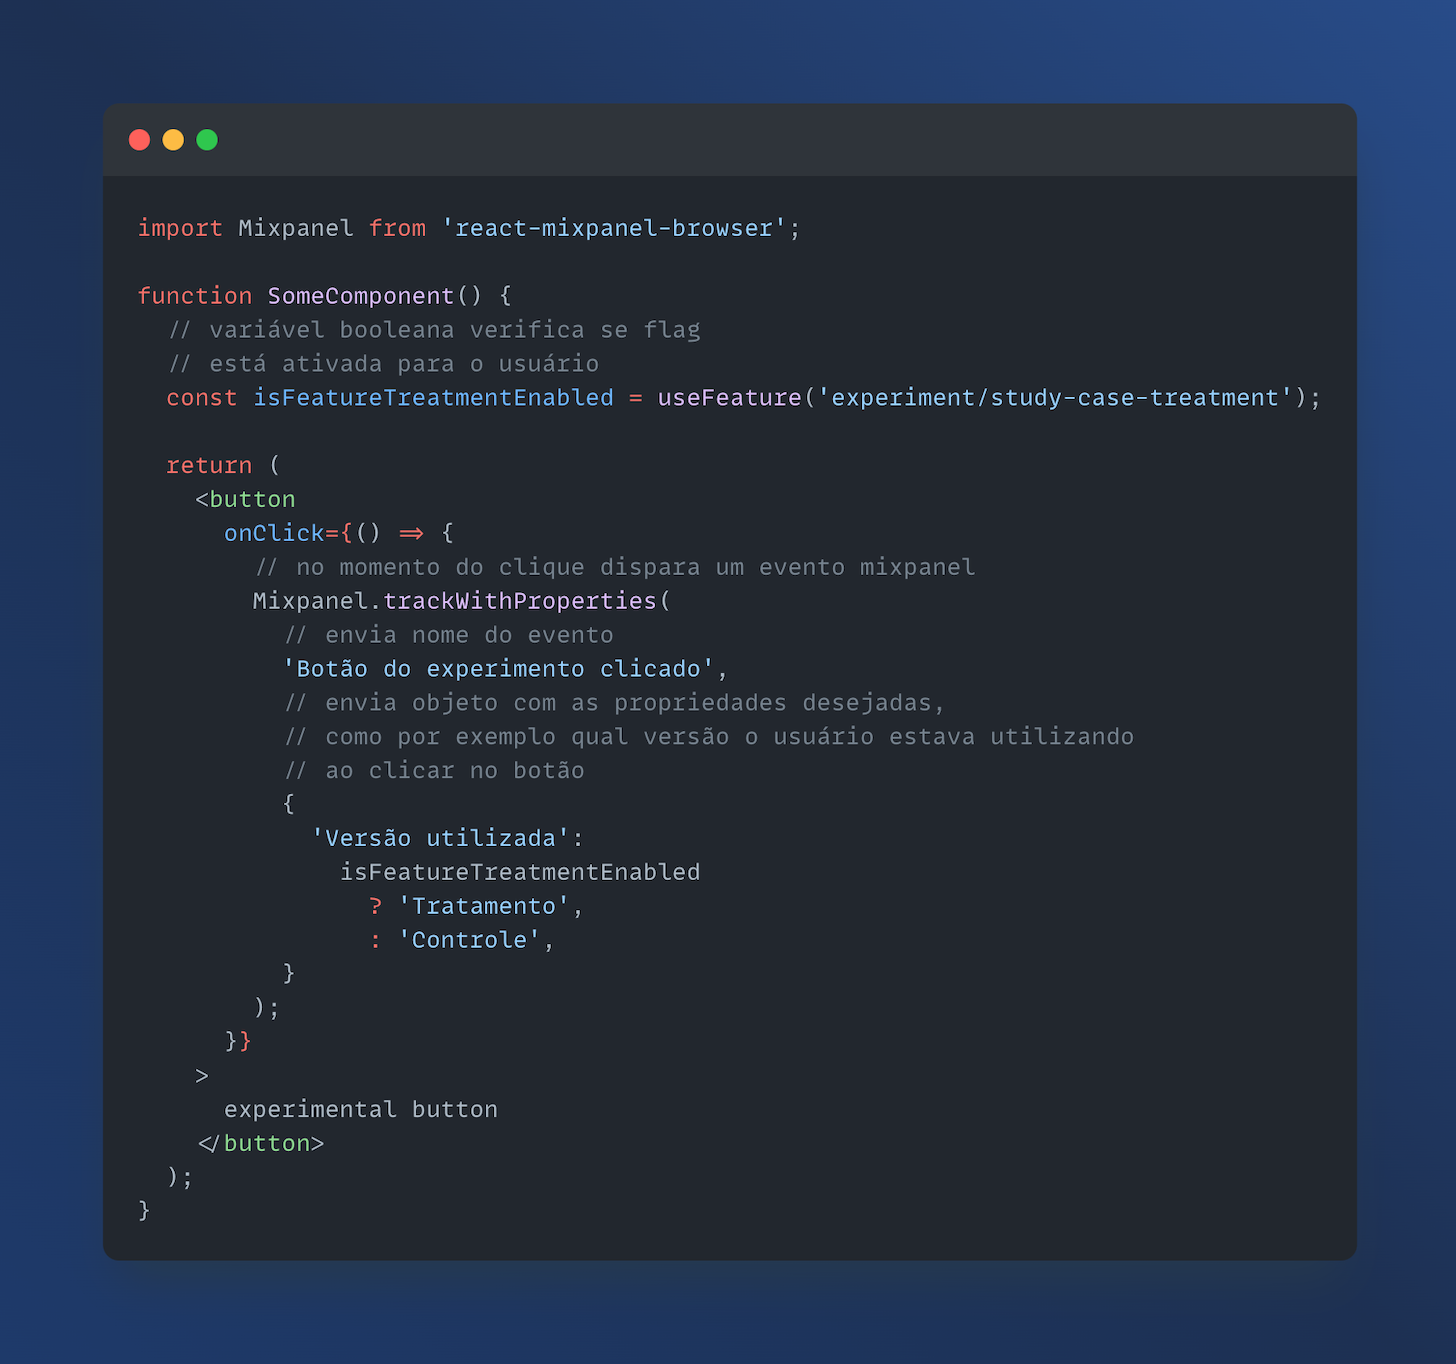
\includegraphics[width=0.75\linewidth]{figuras/exemplo_mixpanel.png}
    \begin{center}
        \text{Fonte: Autor}
    \end{center}
    \label{fig:exemplo-mixpanel-cliente}
\end{figure}

\begin{figure}
    \centering
    \caption{Exemplo de Consumo da API do MixPanel}
    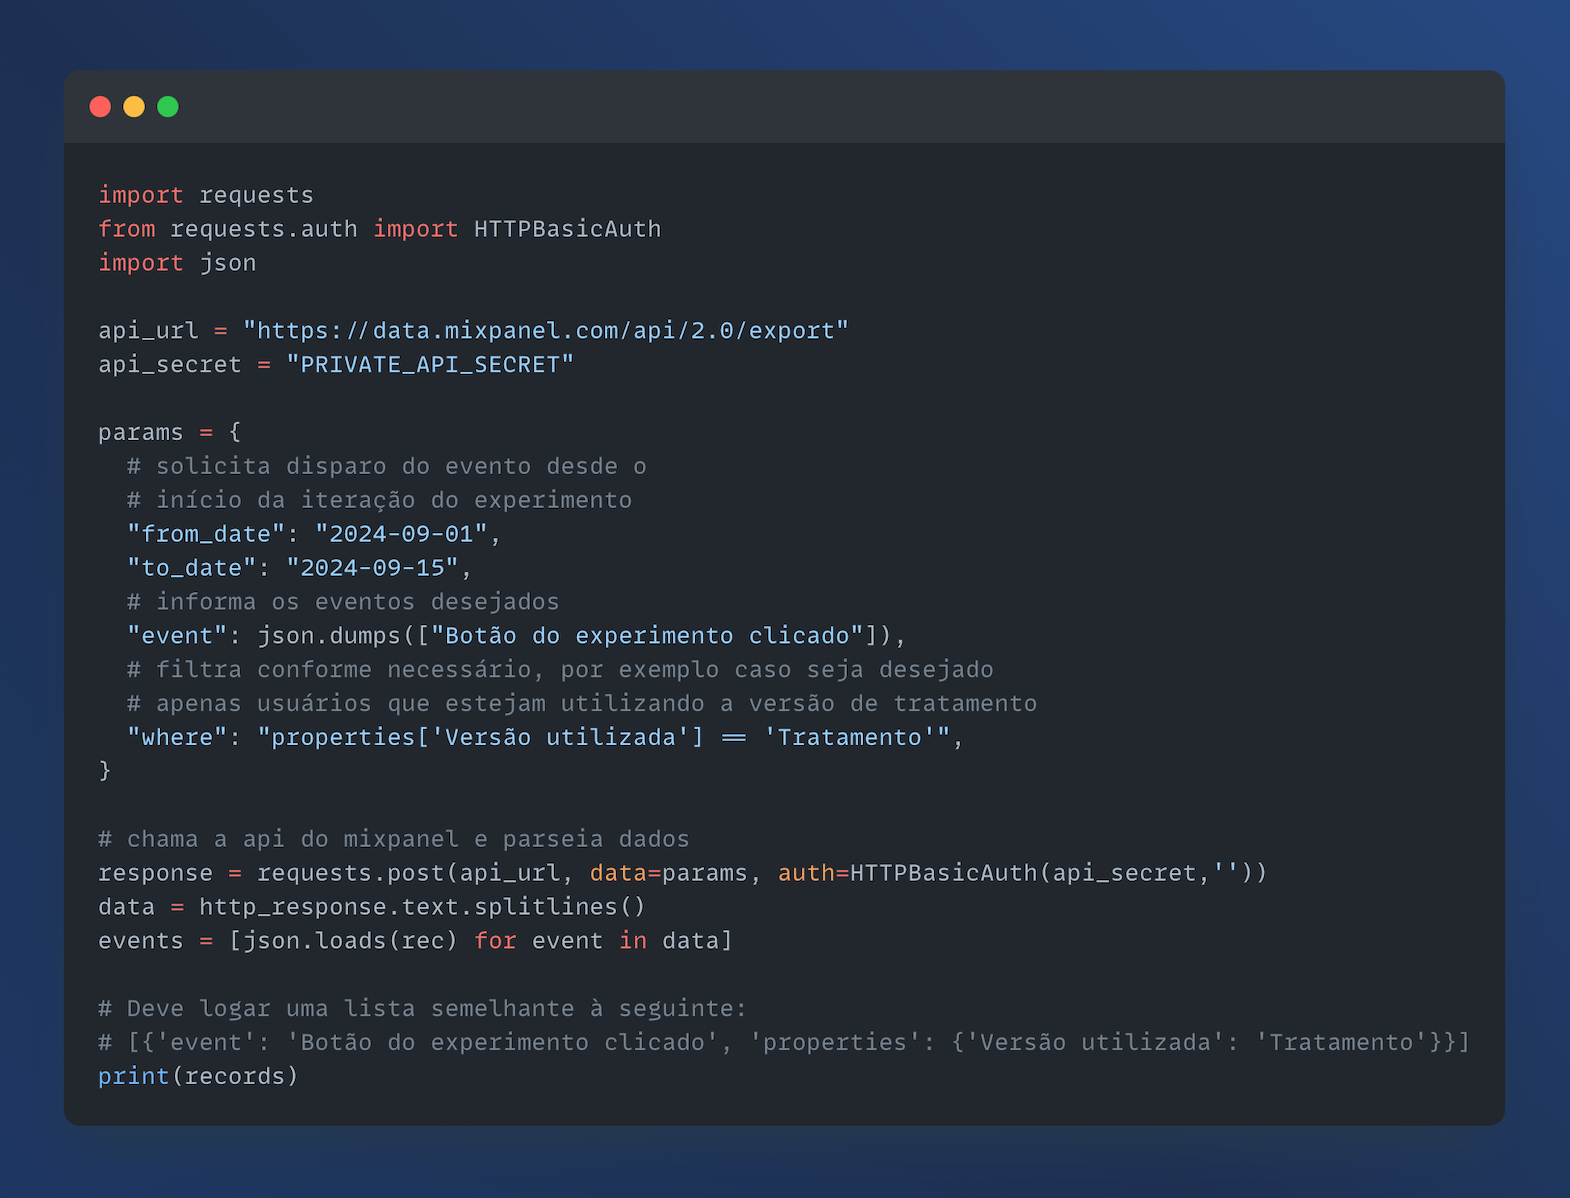
\includegraphics[width=0.75\linewidth]{figuras/exemplo_mixpanel_consumo.png}
    \begin{center}
        \text{Fonte: Autor}
    \end{center}
    \label{fig:exemplo-mixpanel-consumo}
\end{figure}

\subsection{Notion}

O Notion é uma plataforma multifuncional que combina funcionalidades de anotação, criação de documentos estruturados, dashboards personalizados, entre outras \cite{notion}. A ferramenta já é utilizada na empresa para centralizar documentações e dados, permitindo o acesso por todos os colaboradores.

Neste estudo de caso, o Notion será utilizado para documentar as hipóteses e experimentos, registrando os aprendizados. A plataforma servirá para gerenciar e armazenar as hipóteses geradas e priorizadas, assim como os resultados do experimento realizado na segunda etapa do trabalho. Além disso, será elaborado um guia para execução do experimento, a fim de colaborar com futuras experimentações.

\subsection{Python}

Python é uma linguagem de programação aberta conhecida por ser amigável, flexível e de fácil aprendizado \cite{python}. Por causa destas características, a linguagem conta com várias bibliotecas criadas pela comunidade. Dentre elas, diversas que possibilitam o uso de técnicas de estatística descritiva, bem como a realização de testes estatísticos.

No contexto deste trabalho, Python será utilizado para desenvolver \textit{scripts} que irão recuperar os eventos de uso da plataforma MixPanel conforme necessário, além de auxiliar as análises e testes estatísticos. A Figura \ref{fig:python} apresenta um exemplo onde a linguagem é utilizada para essas atividades.


\begin{figure}
    \centering
    \caption{Exemplo de Utilização do Python Para Análise de Dados}
    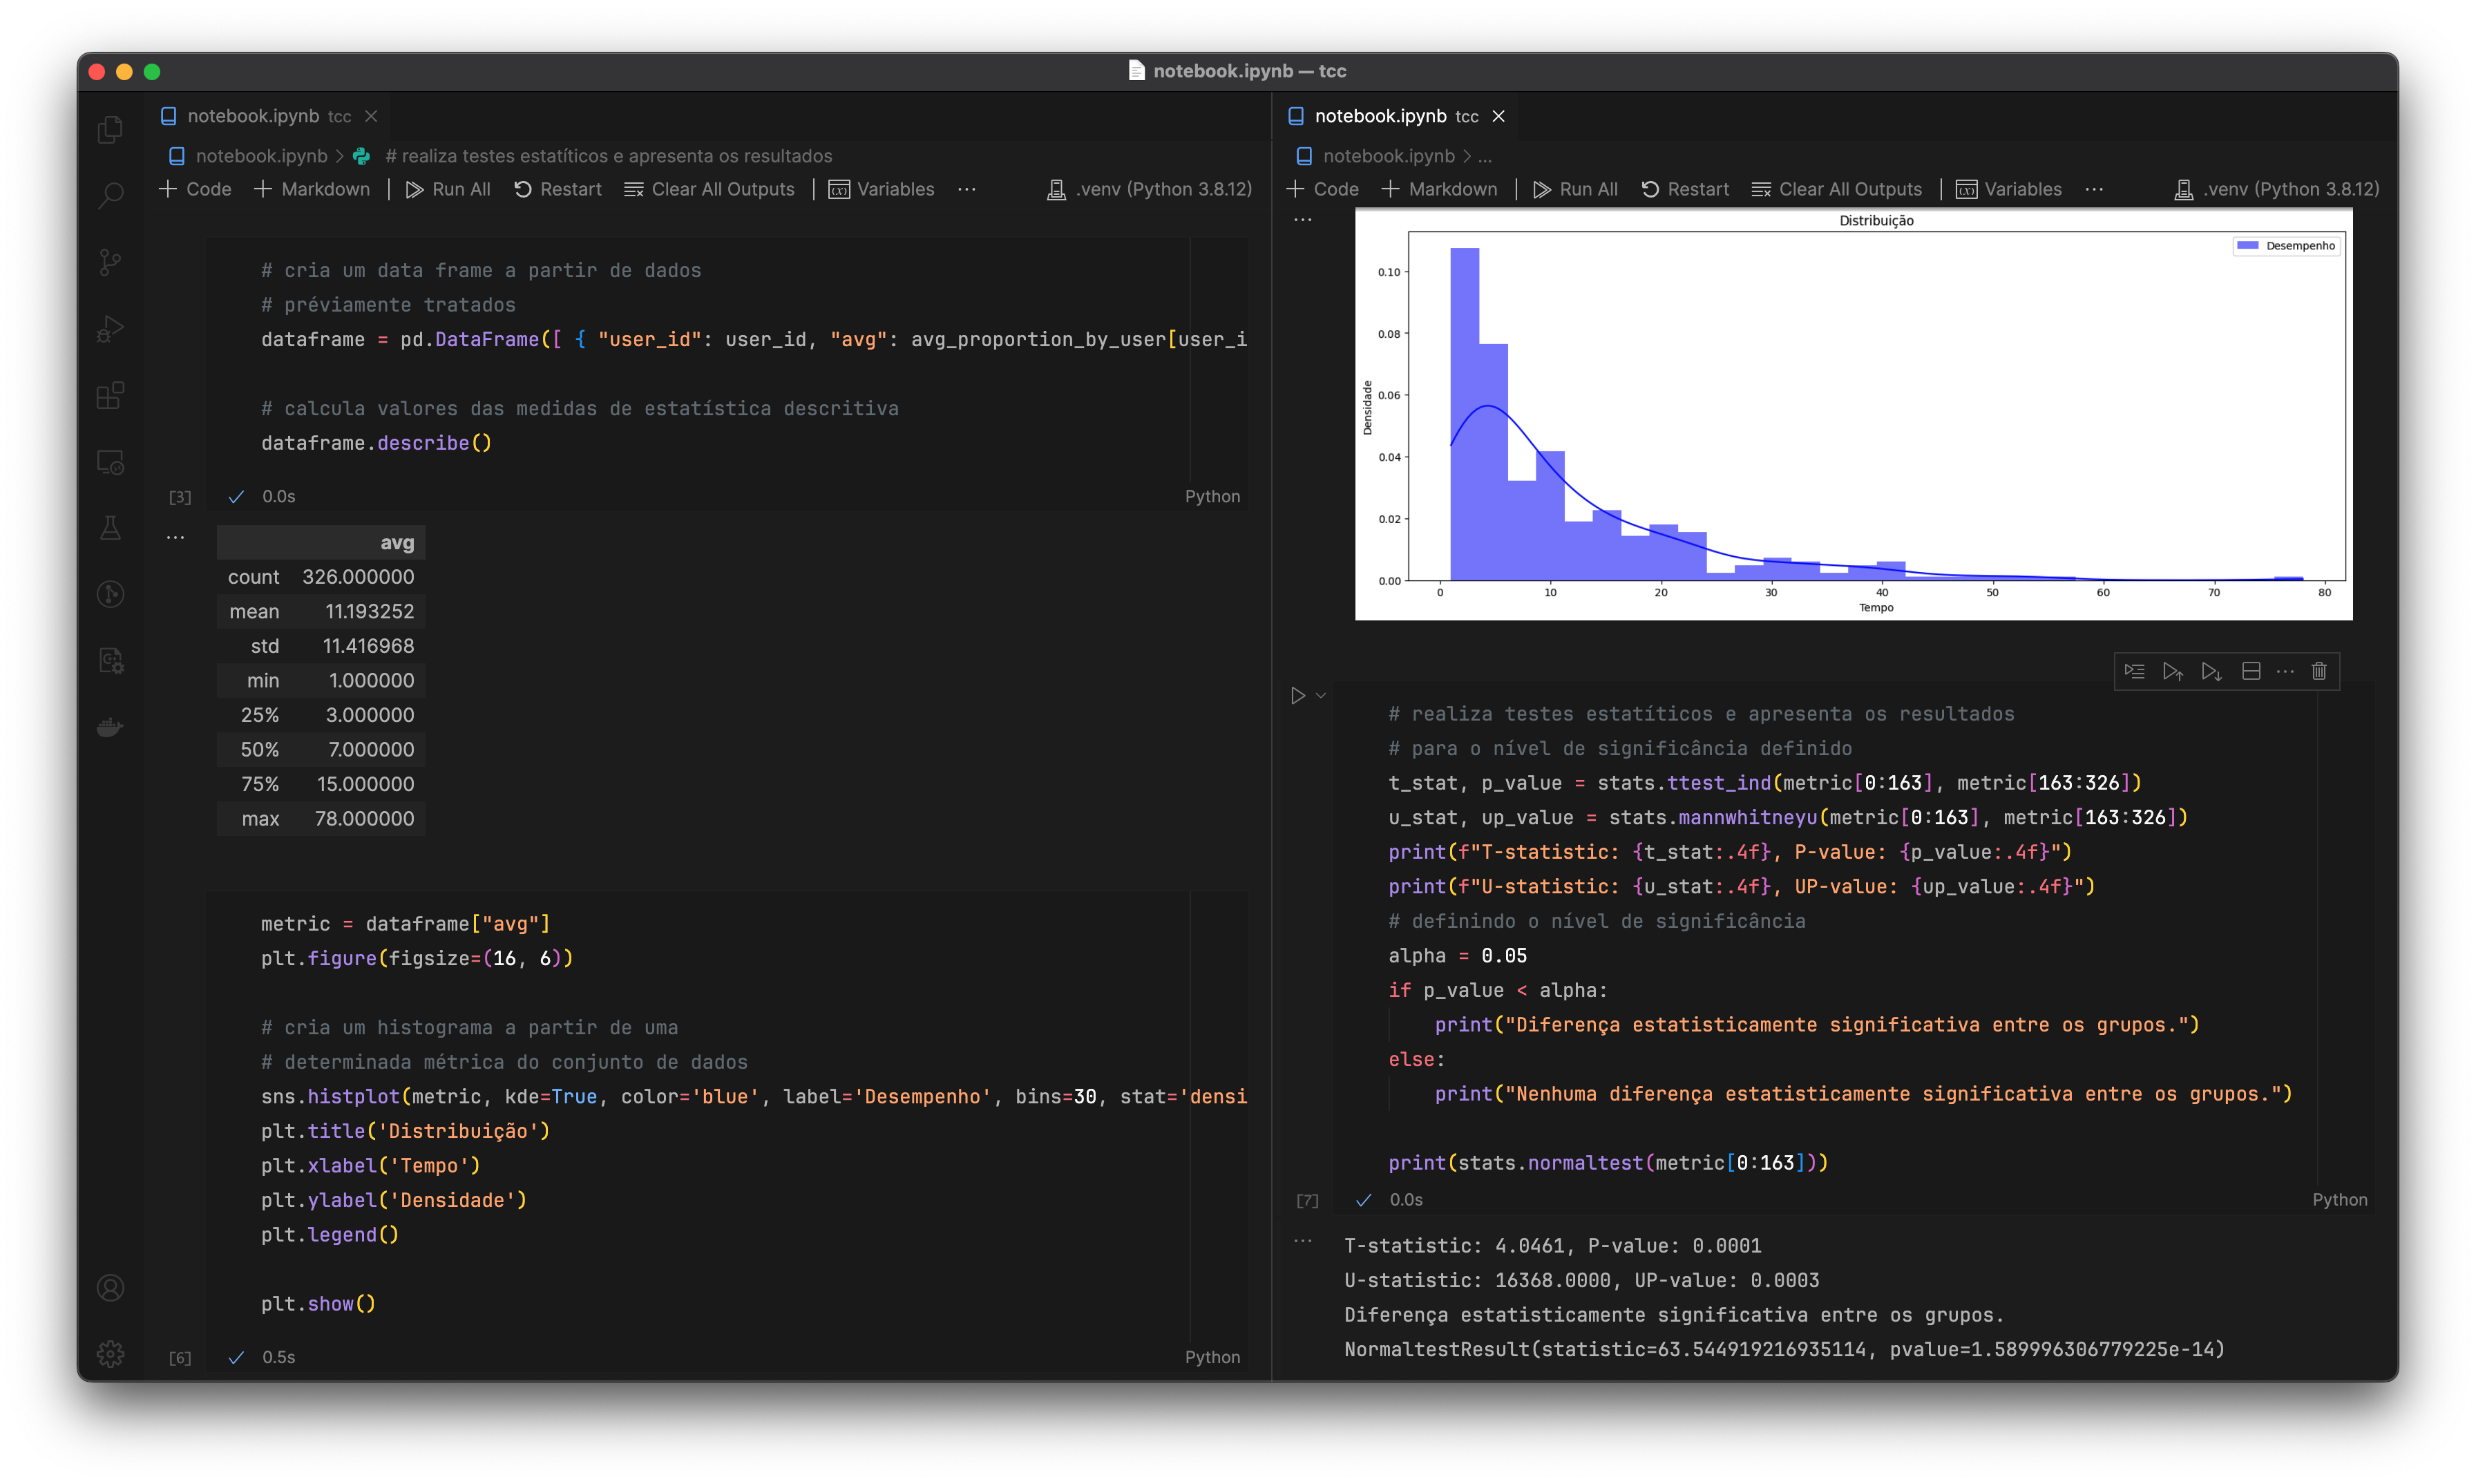
\includegraphics[width=1\linewidth]{figuras/python.png}
    \begin{center}
        \text{Fonte: Autor}
    \end{center}
    \label{fig:python}
\end{figure}